\documentclass[border=6pt]{standalone}
\usepackage[utf8]{inputenc}
\usepackage[T1]{fontenc}
\usepackage{varwidth}
\usepackage{tikz}
\usetikzlibrary{calc,backgrounds}
\renewcommand{\familydefault}{\sfdefault}
\tikzset{
  bot/.style={rectangle, rounded corners=6pt, fill=white, draw=black!25, inner sep=5pt, align=left},
  pac/.style={rectangle, rounded corners=6pt, fill=green!12, draw=green!45!black!40, inner sep=5pt, align=left},
}
\begin{document}
\small\hyphenpenalty=10000\exhyphenpenalty=10000
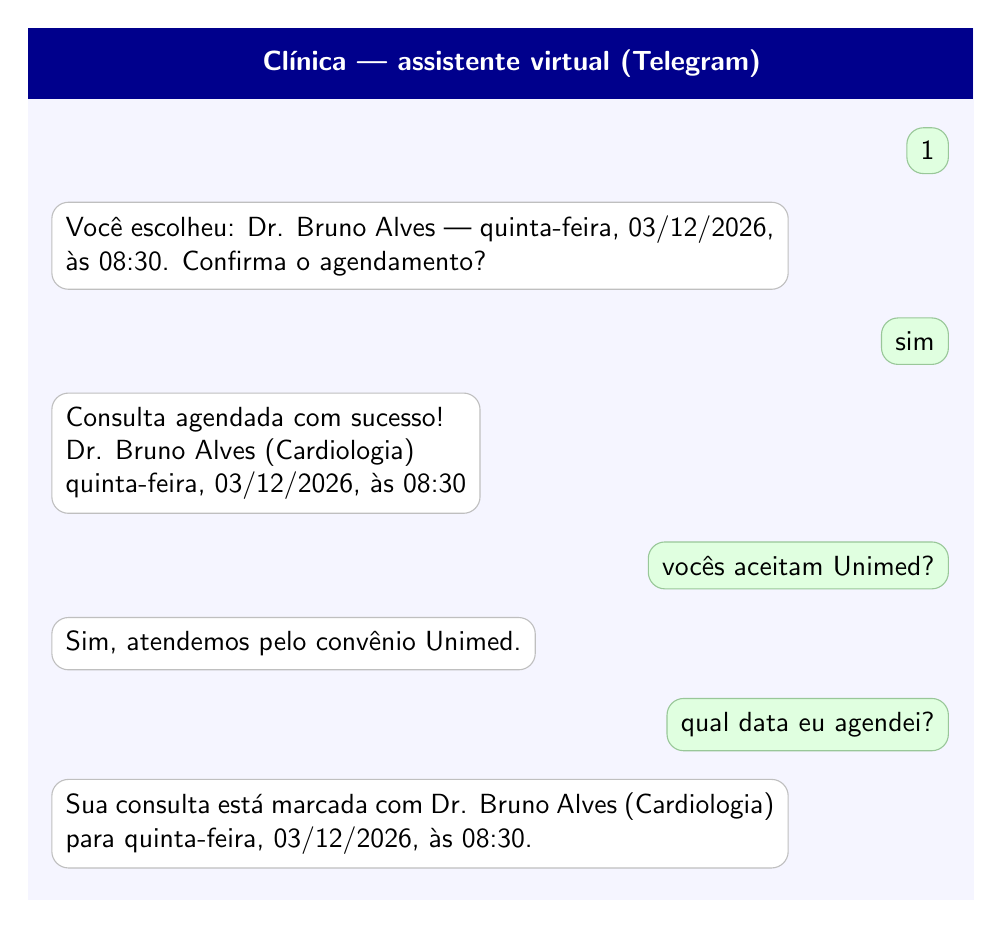
\begin{tikzpicture}
\def\W{12}
\node[anchor=north west, fill=blue!55!black, text=white, minimum width=\W cm, minimum height=0.9cm,
      inner sep=0pt, font=\bfseries] (topo) at (0,0) {\hspace{8pt}Clínica — assistente virtual (Telegram)};
\coordinate (dir) at ({\W-0.3},0);
\coordinate (esq) at (0.3,0);

\path (topo.south) ++(0,-3.5mm) coordinate (c1);
\node[pac, anchor=north east] (m1) at (dir |- c1) {\begin{varwidth}{7.5cm}1\end{varwidth}};
\path (m1.south) ++(0,-3.5mm) coordinate (c2);
\node[bot, anchor=north west] (m2) at (esq |- c2) {\begin{varwidth}{9cm}Você escolheu: Dr. Bruno Alves — quinta-feira, 03/12/2026, às 08:30. Confirma o agendamento?\end{varwidth}};
\path (m2.south) ++(0,-3.5mm) coordinate (c3);
\node[pac, anchor=north east] (m3) at (dir |- c3) {\begin{varwidth}{7.5cm}sim\end{varwidth}};
\path (m3.south) ++(0,-3.5mm) coordinate (c4);
\node[bot, anchor=north west] (m4) at (esq |- c4) {\begin{varwidth}{9cm}Consulta agendada com sucesso!\\Dr. Bruno Alves (Cardiologia)\\quinta-feira, 03/12/2026, às 08:30\end{varwidth}};
\path (m4.south) ++(0,-3.5mm) coordinate (c5);
\node[pac, anchor=north east] (m5) at (dir |- c5) {\begin{varwidth}{7.5cm}vocês aceitam Unimed?\end{varwidth}};
\path (m5.south) ++(0,-3.5mm) coordinate (c6);
\node[bot, anchor=north west] (m6) at (esq |- c6) {\begin{varwidth}{9cm}Sim, atendemos pelo convênio Unimed.\end{varwidth}};
\path (m6.south) ++(0,-3.5mm) coordinate (c7);
\node[pac, anchor=north east] (m7) at (dir |- c7) {\begin{varwidth}{7.5cm}qual data eu agendei?\end{varwidth}};
\path (m7.south) ++(0,-3.5mm) coordinate (c8);
\node[bot, anchor=north west] (m8) at (esq |- c8) {\begin{varwidth}{9cm}Sua consulta está marcada com Dr. Bruno Alves (Cardiologia) para quinta-feira, 03/12/2026, às 08:30.\end{varwidth}};
\path (m8.south) ++(0,-4mm) coordinate (fim);
\begin{scope}[on background layer]
  \fill[blue!4] (topo.north west) rectangle (topo.east |- fim);
\end{scope}
\end{tikzpicture}
\end{document}
